\newpage
\section{Simulation Analysis}
\label{sec:simulation}
Since the input voltage source in this circuit is sinusoidal, the voltage and current values of the various components vary in time, and we are interested therefore in analysing how they evolve in time and obviously we want to picture the transformation of our AC input voltage source throughout the multiple stages of the circuit. Therefore, we will run a single transient analysis for this circuit, lasting 10 periods of the voltage source. For this simulation we are not taking the natural solution into account, only the forced one. In our simulation we came across a large transitional period of roughly 4 seconds, until the output voltage source stabilized enough in the envelope detector, so we only account for data after this period, [3.8 ; 4.0]. This is due to the natural solution of the voltage and its downfall effects will be aproached in our conclusions. We used the default diode model of NGSpice in this simulation and we saw no need of introducing a transformer since it only reduces the amplitude of the voltage source, so we applied the AC voltage output of the transformer as our input voltage source of the circuit.
\subsection{Envelope Detector Output Voltage}
In figure~\ref{fig:envelope} we present the plot of the envelope detector output voltage throughout 10 periods, and in table~\ref{tab:envelope} we introduce the average voltage (approximate DC component) and the voltage ripple of such voltage. Since the objective lies in the output of the regulator, this set of data isn't of much relevance.

\begin{figure}[!h] \centering
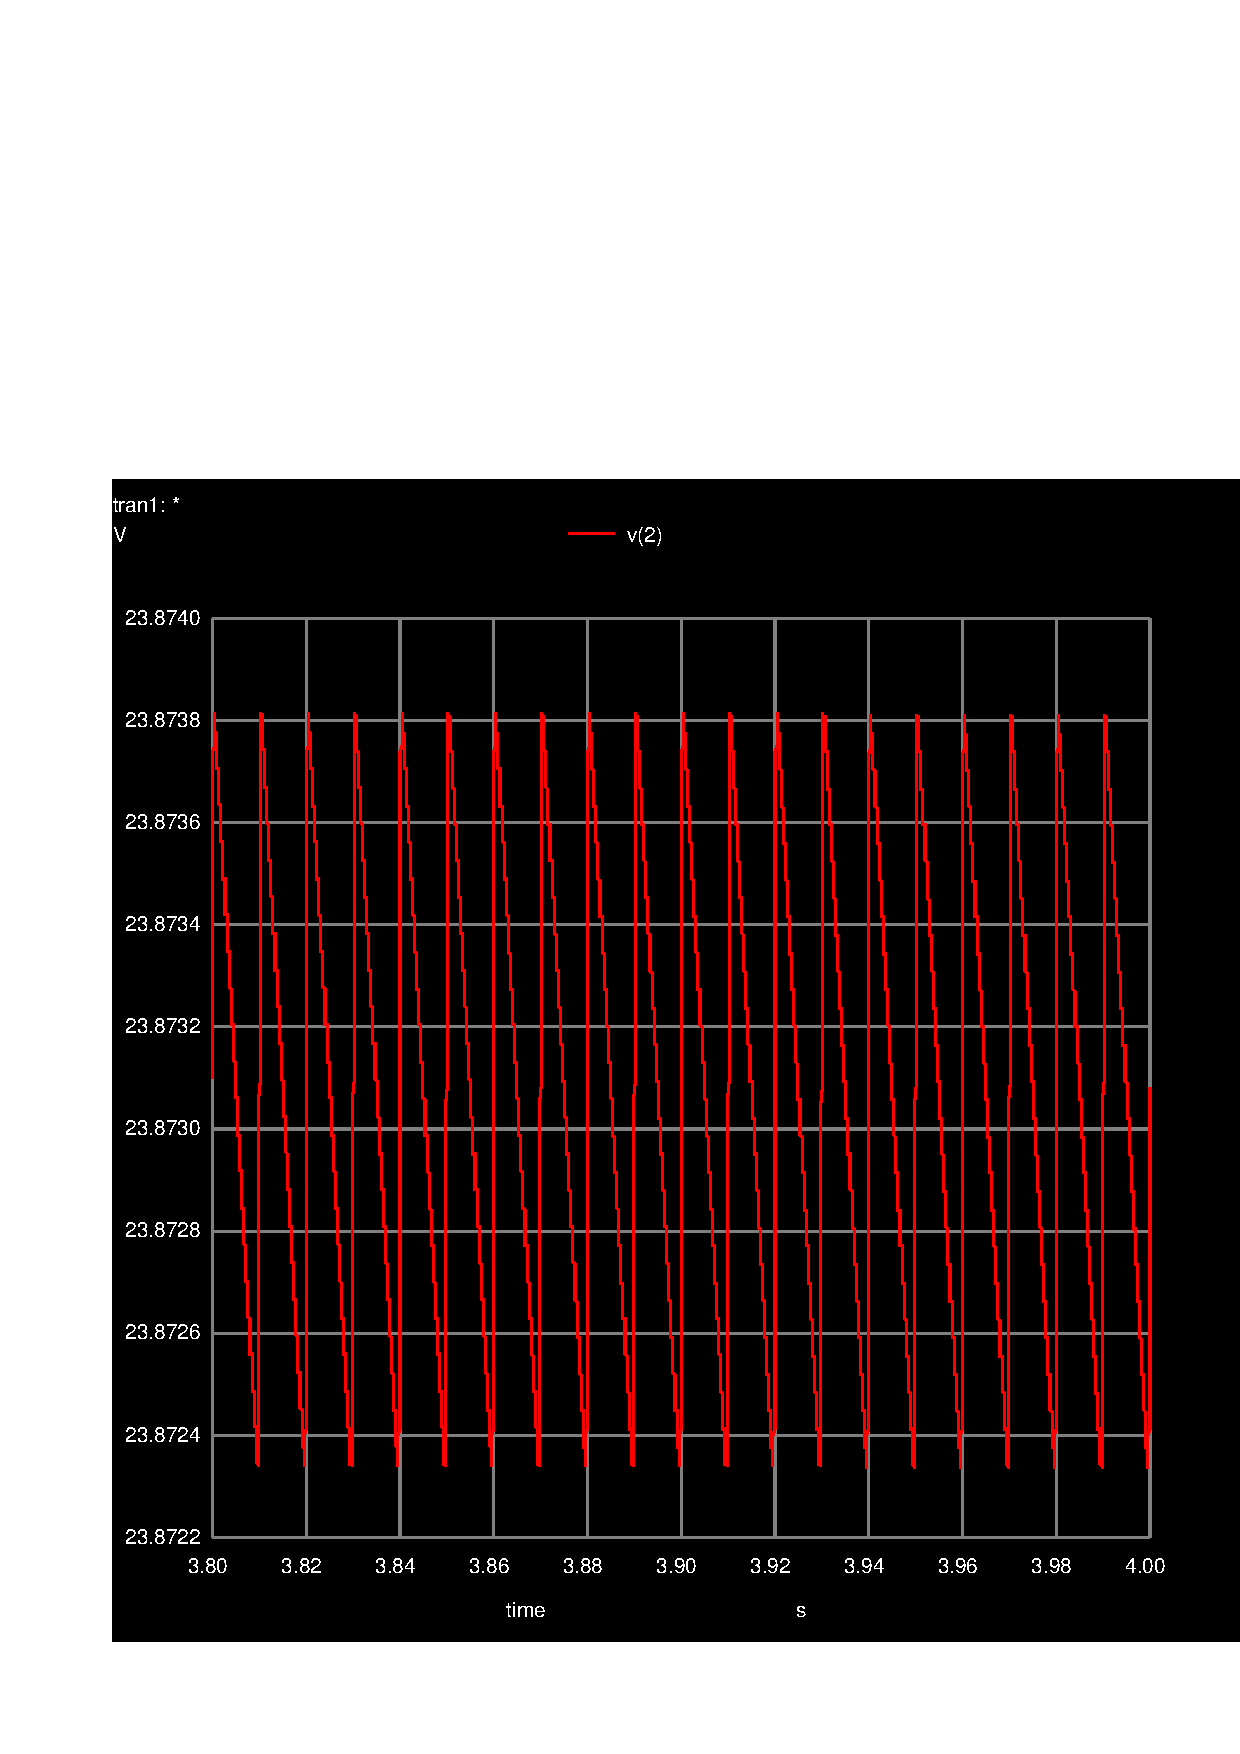
\includegraphics[width=0.6\linewidth]{envelope.pdf}
\caption{Simulated output voltage in the envelope detector.}
\label{fig:envelope}
\end{figure}

\begin{table}[h]
  \centering
  \begin{tabular}{|l|r|}
    \hline    
    {\bf Name} & {\bf Values [V]} \\ \hline
    \input{env_tab} 
  \end{tabular}
  \caption{Envelope Detector Output Voltage characteristics.}
  \label{tab:envelope}
\end{table}

\subsection{Voltage Regulator Output Voltage - The output of the circuit}
Now, in figure~\ref{fig:regulator} we present the plot of the voltage regulator output voltage throughout the same 10 periods, and in table~\ref{tab:result} we introduce the average voltage (approximate DC component) and the voltage ripple of such voltage. This is indeed our desired output voltage for the circuit, so its average and ripple are very important data. In this case, we managed a average output voltage that only differs from 12V in its last significant algharism, and a voltage ripple in the order of the uV, which seems to us a pretty satisfactory result.

\begin{figure}[!h] \centering
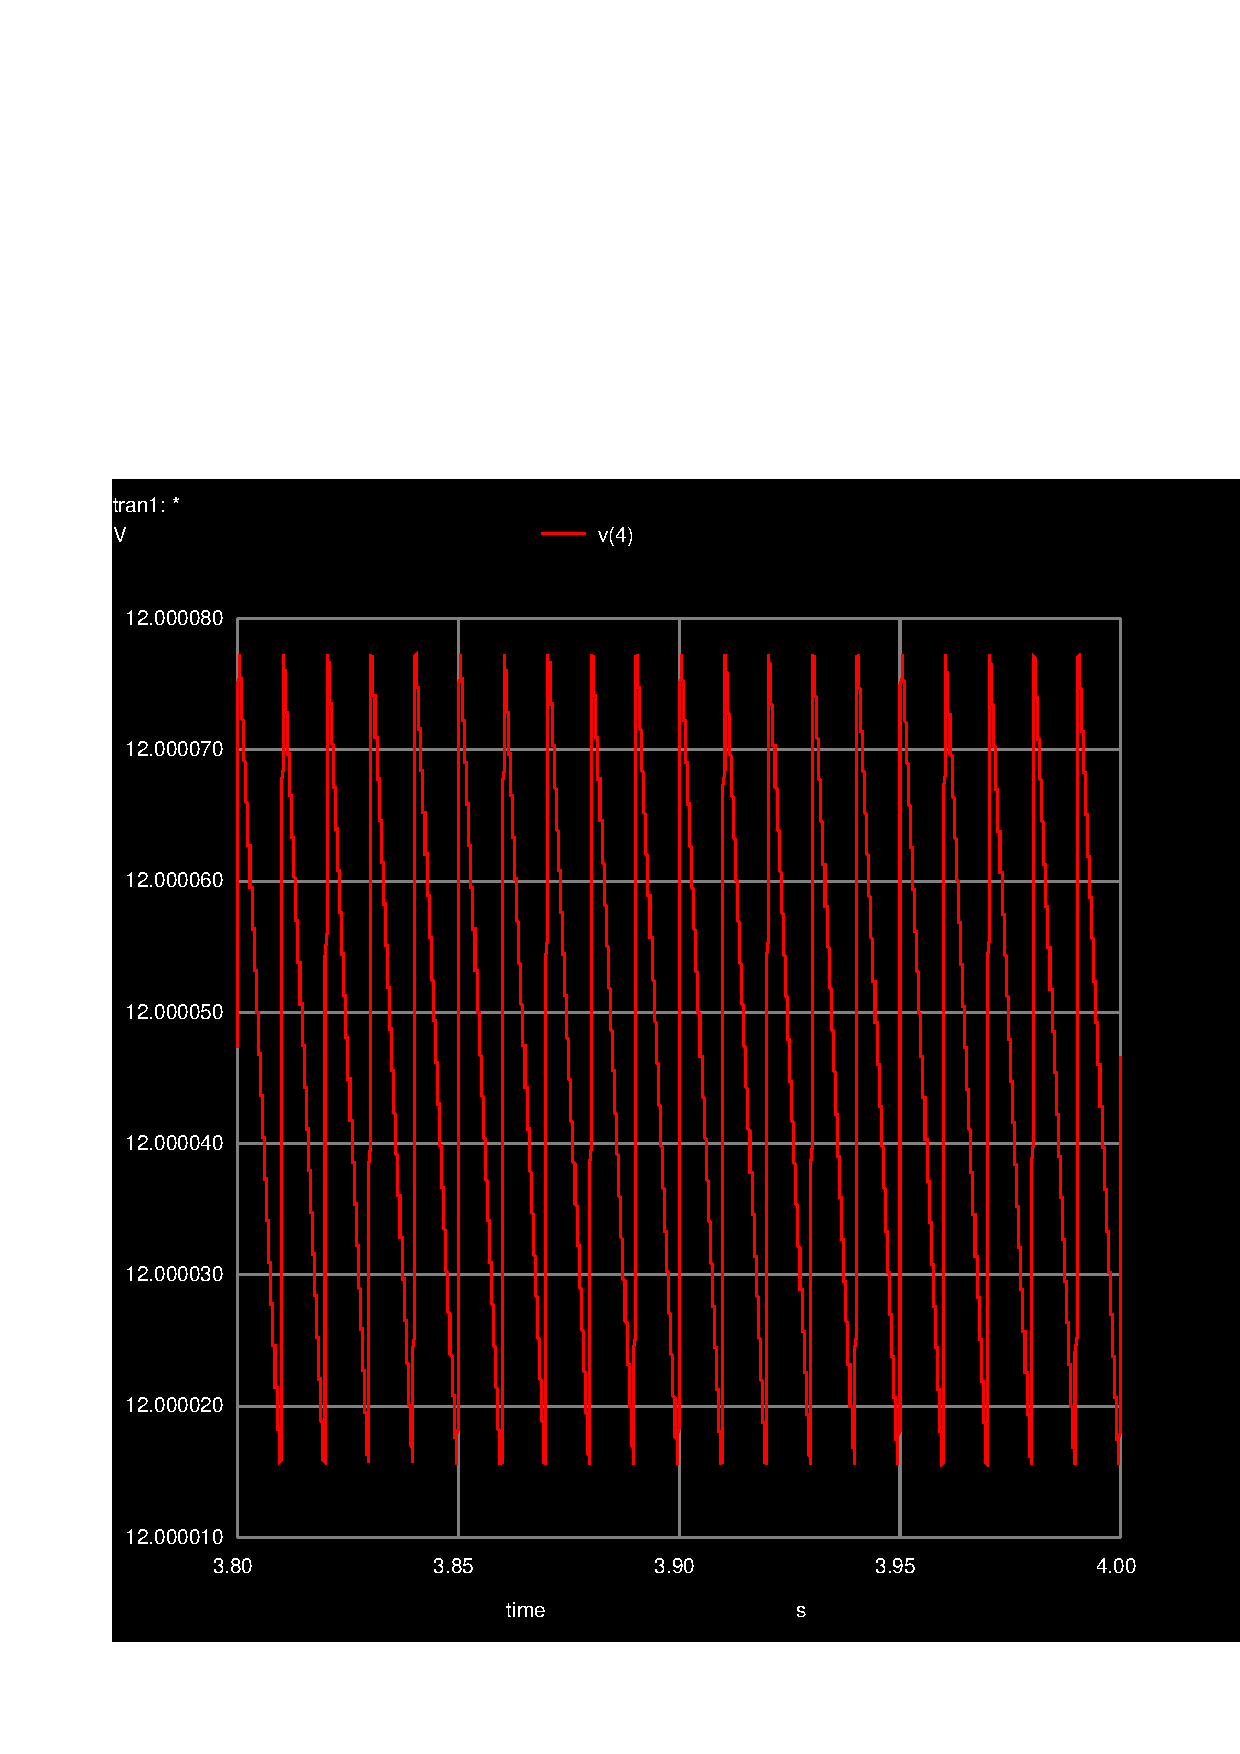
\includegraphics[width=0.6\linewidth]{regulator.pdf}
\caption{Simulated output voltage in the voltage regulator.}
\label{fig:regulator}
\end{figure}

\begin{table}[h]
  \centering
  \begin{tabular}{|l|r|}
    \hline    
    {\bf Name} & {\bf Values [V]} \\ \hline
    \input{result_tab} 
  \end{tabular}
  \caption{Voltage Regulator Output Voltage characteristics, and figure of merit.}
  \label{tab:result}
\end{table}

In figure~\ref{fig:deviation} we are able to get a closer look to the slight deviations from the desired linear 12V in our output, and in figure~\ref{fig:total} we compare the input voltage source post-transformer, the output of the envelope detector, and our final output - the voltage regulator output voltage. In this figure we can see the linear character of the voltage post-envelope detector, opposed to its sinusoidal form after the transformer, so the envelope did its job in annihilating the sinusoidal wave form. Then, we can see that our final output voltage maintains this linear (DC) trait, even improving on it thanks to the resistor, and it is now at the desired 12V fruit of the action of our limiter, the 20 diodes in series.

\begin{figure}[!h] \centering
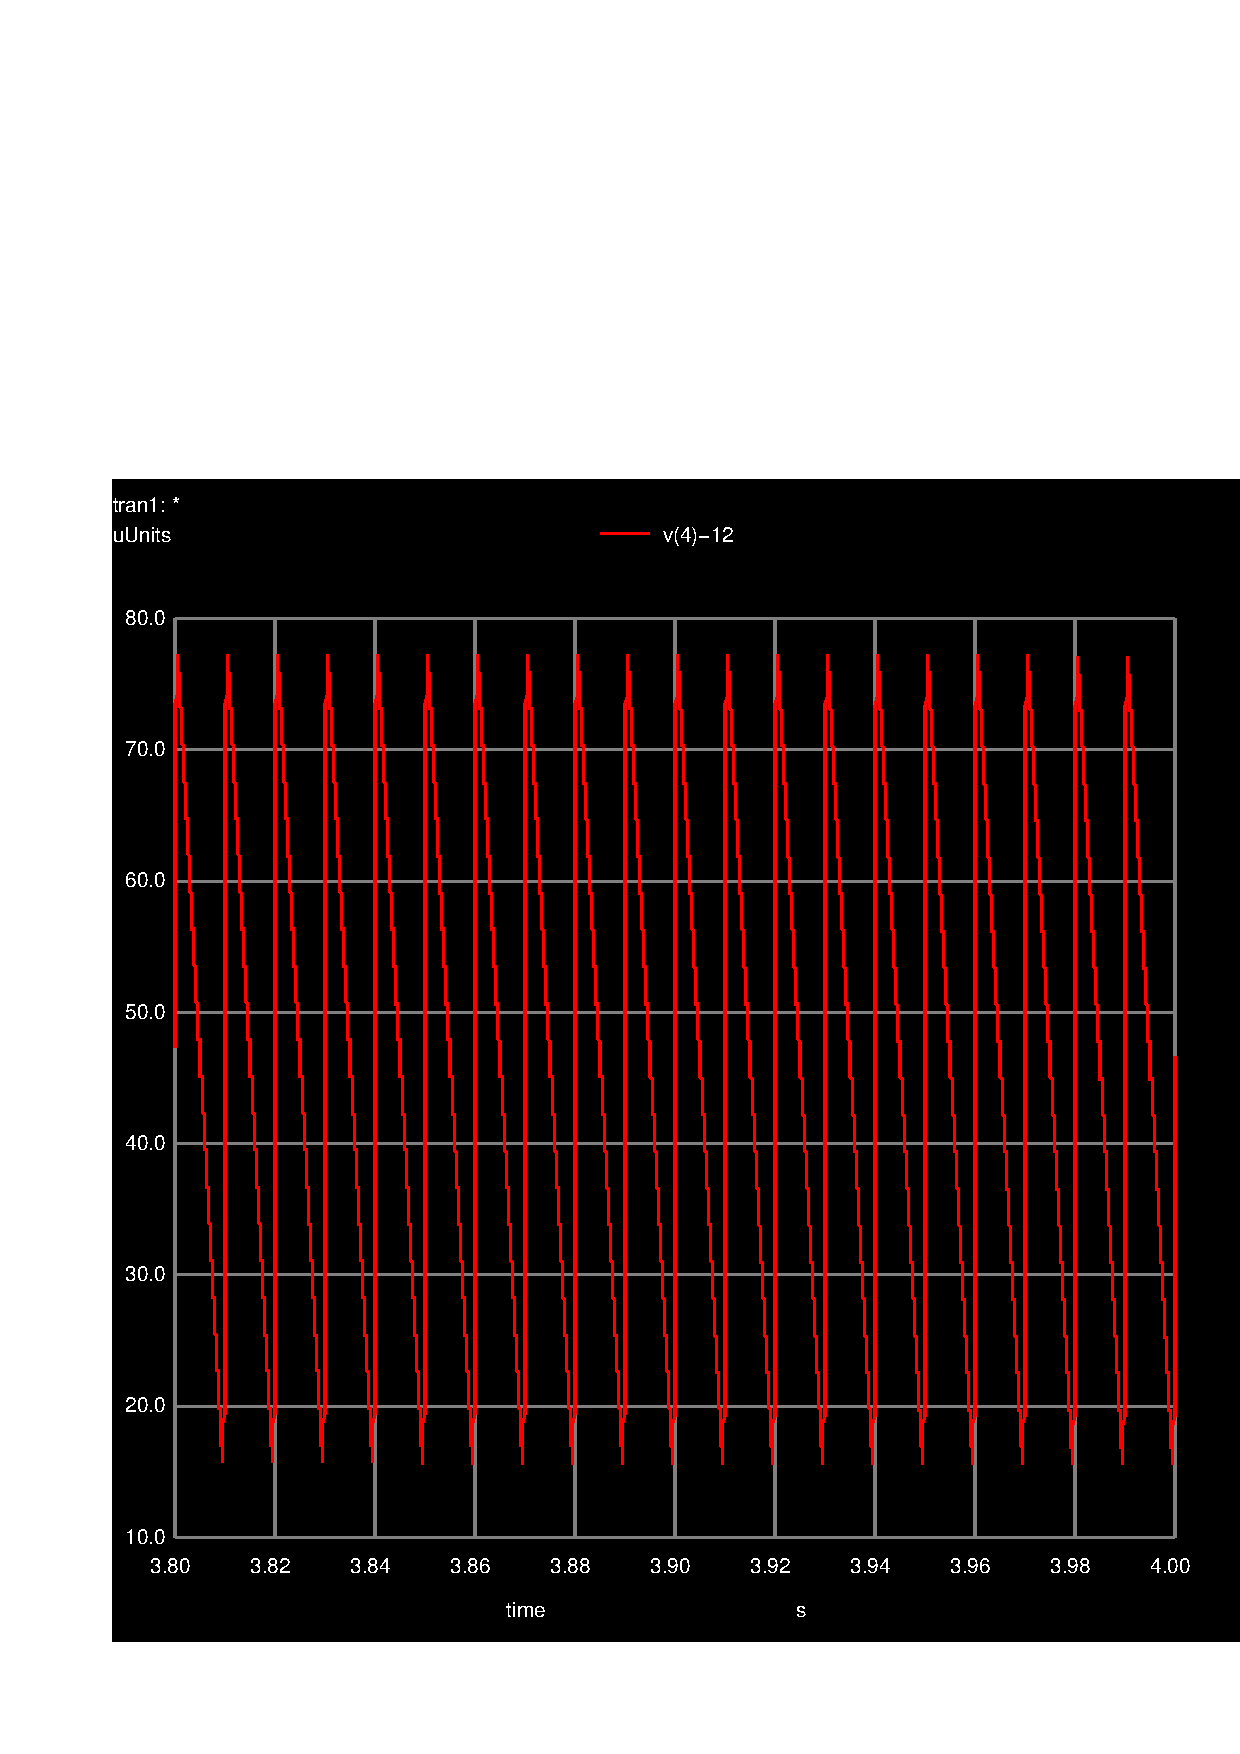
\includegraphics[width=0.6\linewidth]{deviation.pdf}
\caption{Deviation from 12V of the output voltage in the voltage regulator.}
\label{fig:deviation}
\end{figure}

\begin{figure}[!h] \centering
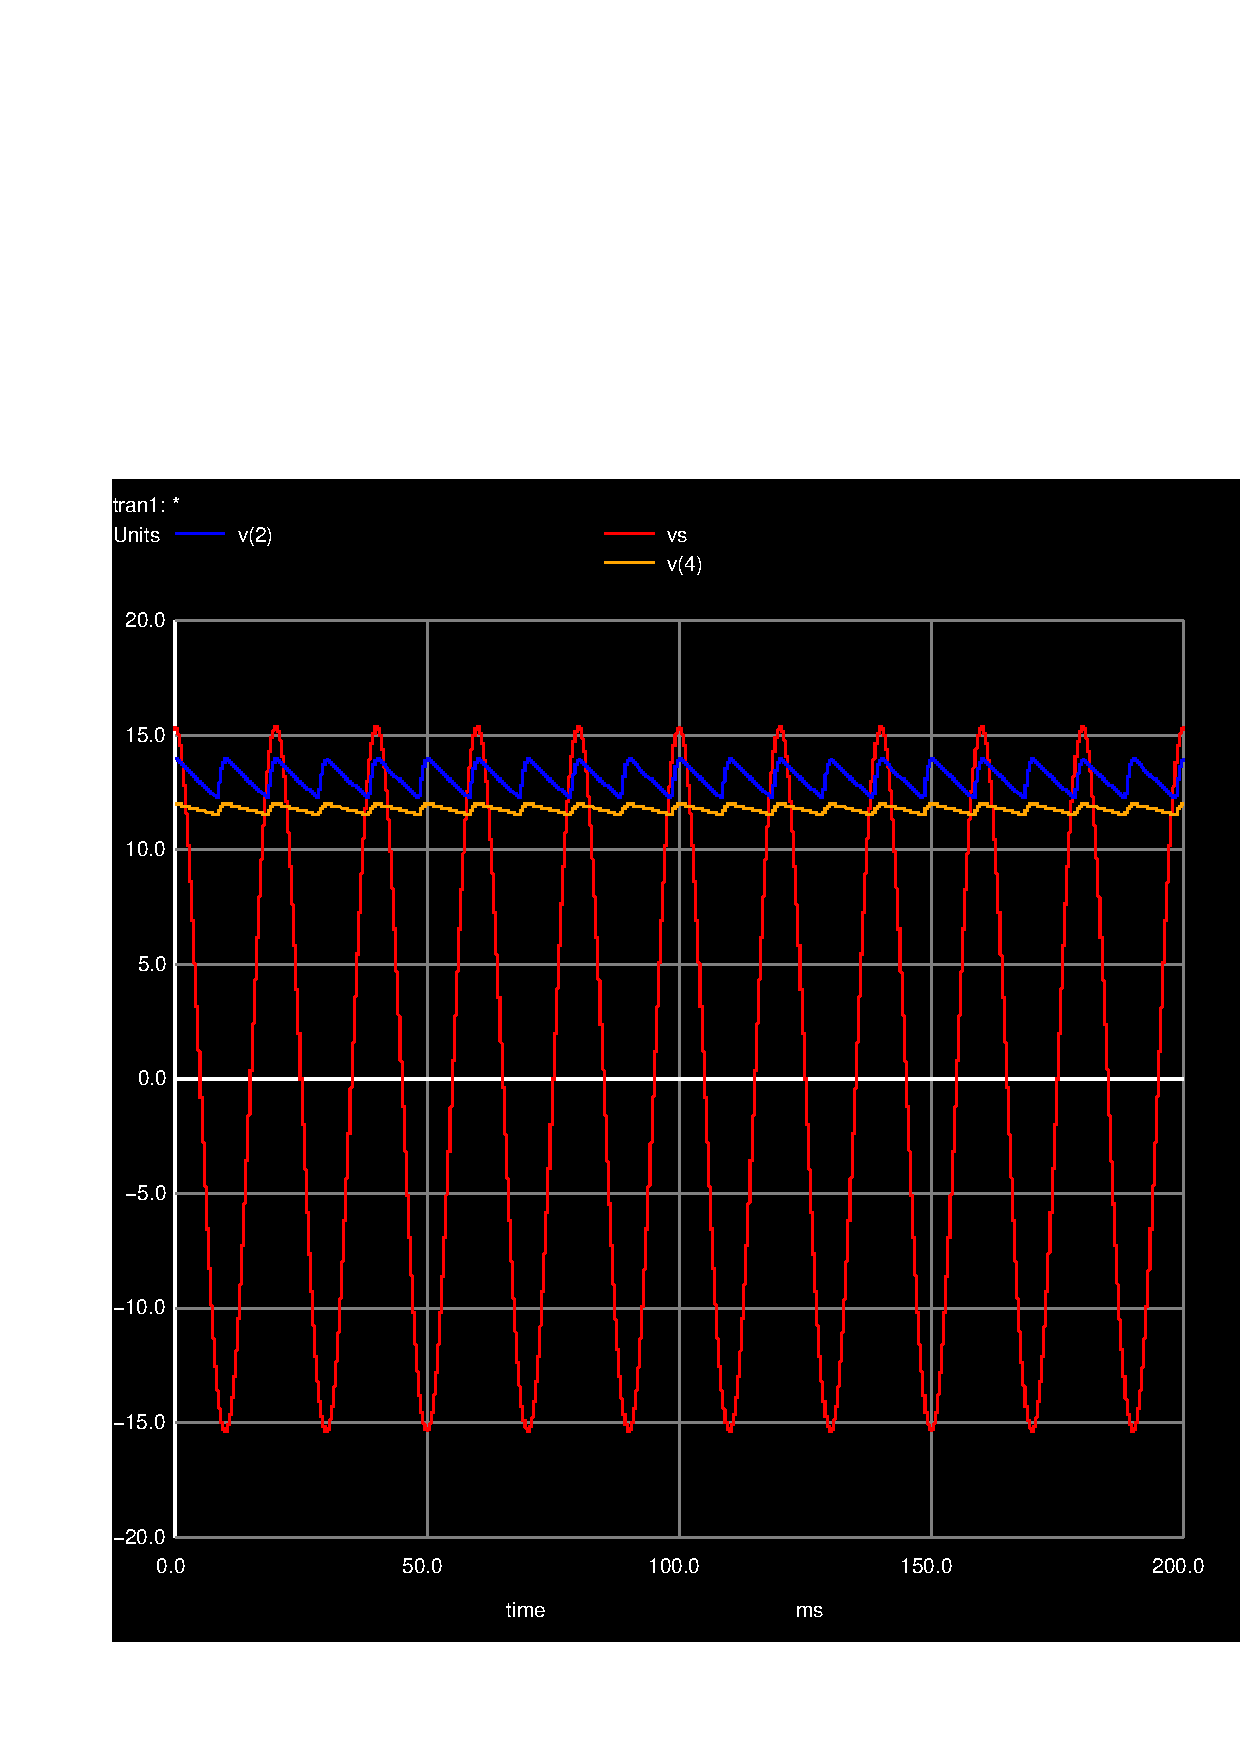
\includegraphics[width=0.6\linewidth]{total.pdf}
\caption{Comparison of the simulated input voltage source (after transformer), the envelope detector voltage and, finally, the voltage regulator voltage, our output.}
\label{fig:total}
\end{figure}

Going back to table~\ref{tab:result}, we calculated the figure of merit for this configuration, and obtained a value close to 5. The value could have been higher if the average of the output voltage were a straight 12V, which is not the case. Another way to increase the merit would have been to diminuish our ripple by increasing our resistors and capacitor values. Even though we would be increasing our cost, the decrease of the ripple would have an even bigger effect than that of the cost, increasing our merit. However, we noticed this could come at the cost of a even bigger transitional period, which is not a good model for an AC/DC converter, since it is impractical to wait more than 5 seconds for the conversion to take place in an effective manner. A way to decrease this transitional period could come in the form of increasing the input voltage source coming from the transformer, but that would require an even bigger resistance in the regulator to help bring that value down (we're using the default diode model, not the theoretical ideal one)... Final notes on the figure of merit topic will be approached in our conclusions.

\par
